\subsection{Introduction}
\label{comesh:section:intro}

Commercial edge deployments with Internet of Things (IoT) devices are rapidly growing in size and density. There are over 10 B IoT devices today, expected to exceed 25 B by 2030~\cite{IoTstats}. Commercial settings are the next frontier beyond smart homes (\Cref{comesh:fig:IoTsetting}). For example, smart buildings already account for 1.26 B devices, and are forecast to grow by 2027 to 2.5 B devices and a \$90+ B market~\cite{Memoori}.
Other emerging areas for IoT deployment in  commercial edges include smart farms with sensors and robots~\cite{farmbeats},
Industry 4.0~\cite{lampropoulos2019internet},
battlefields~\cite{IoBT},
and indoor spaces like
warehouses~\cite{fatima2022production}.
Each of these market sectors is growing fairly   quickly~\cite{iotagrimarket}.

Because commercial settings have large physical footprints (unlike smart homes, which are small), it is common 
for them to contain {\it mesh networks} among the IoT devices. Mesh networking technology has matured
using Wifi,
Zigbee, Bluetooth, LoRa, etc.~\cite{sayian}.
Industry commonly uses  IEEE 802.15.4, WirelessHart~\cite{song2008wirelesshart}, or IEC~\cite{iso_central_secretary_systems_2016} to build such IoT meshes.  A mesh network (a.k.a. an ad-hoc network) is robust, resilient,
scalable, and enables
control without requiring a central operating unit (or hub), which may be prohibitive to set up, be overloaded, or prolong latencies. These mesh networks usually contain a mixture of devices that are ``smart'' devices capable of (small amounts of) compute and storage, along with  ``simple'' devices that can only receive commands. 
There is rich literature at the networking layer, e.g., on how to build, configure, and perform routing in mesh networks~\cite{akyildiz2005survey,lynch2024case}.

\begin{figure}[t!]
    \centering
    \begin{subfigure}{0.49\linewidth}
        \centering
        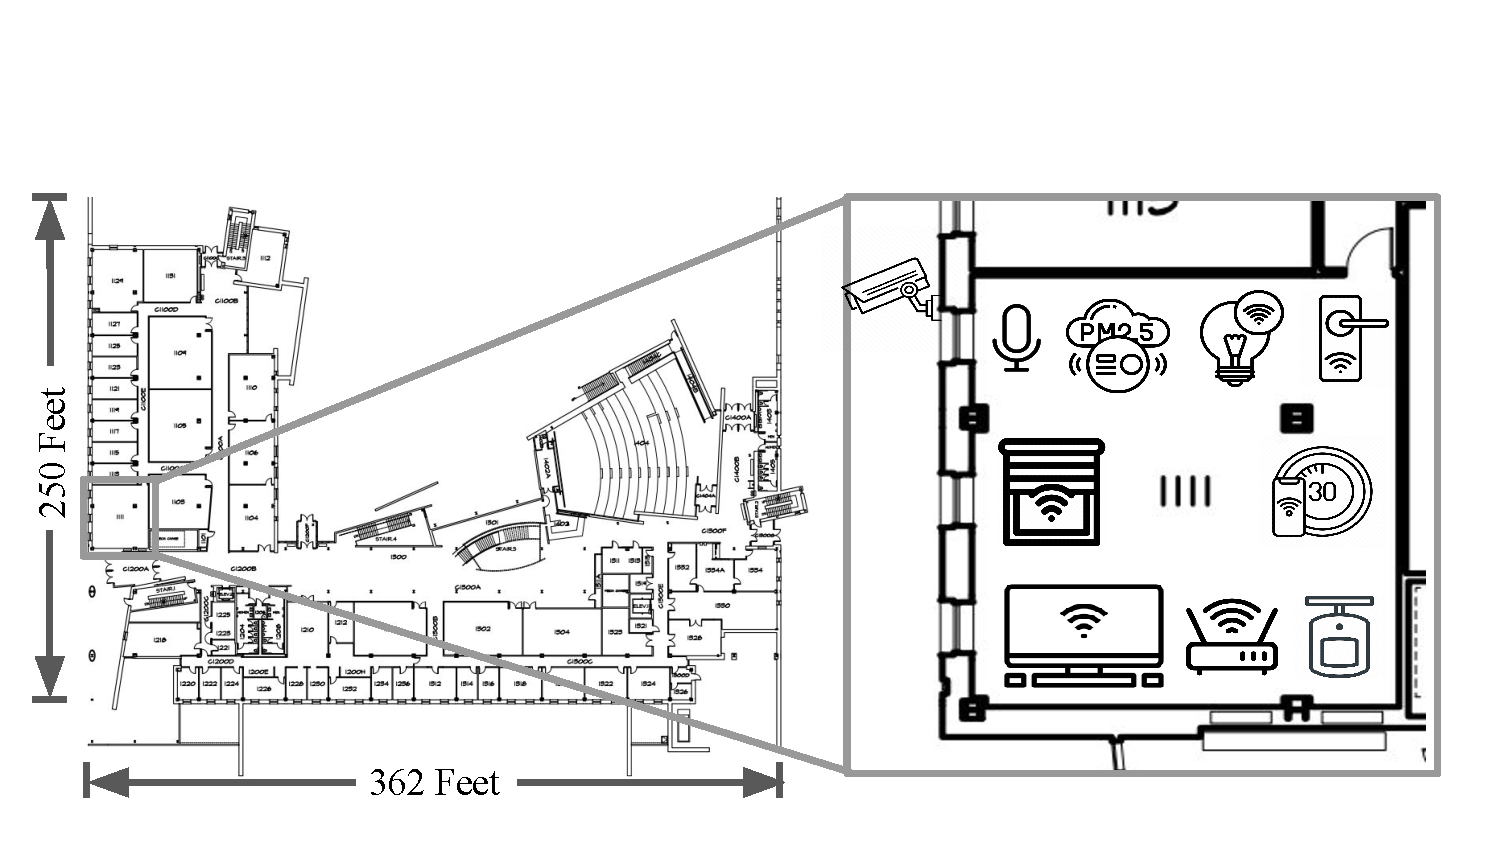
\includegraphics[width=\textwidth]{CoMesh/figures/intro/smart-building.pdf}
        \caption{\it \small {Smart Building.}}
        \medskip
        \label{comesh:fig:smart-building}
    \end{subfigure}
    \begin{subfigure}{0.49\linewidth}
        \centering
        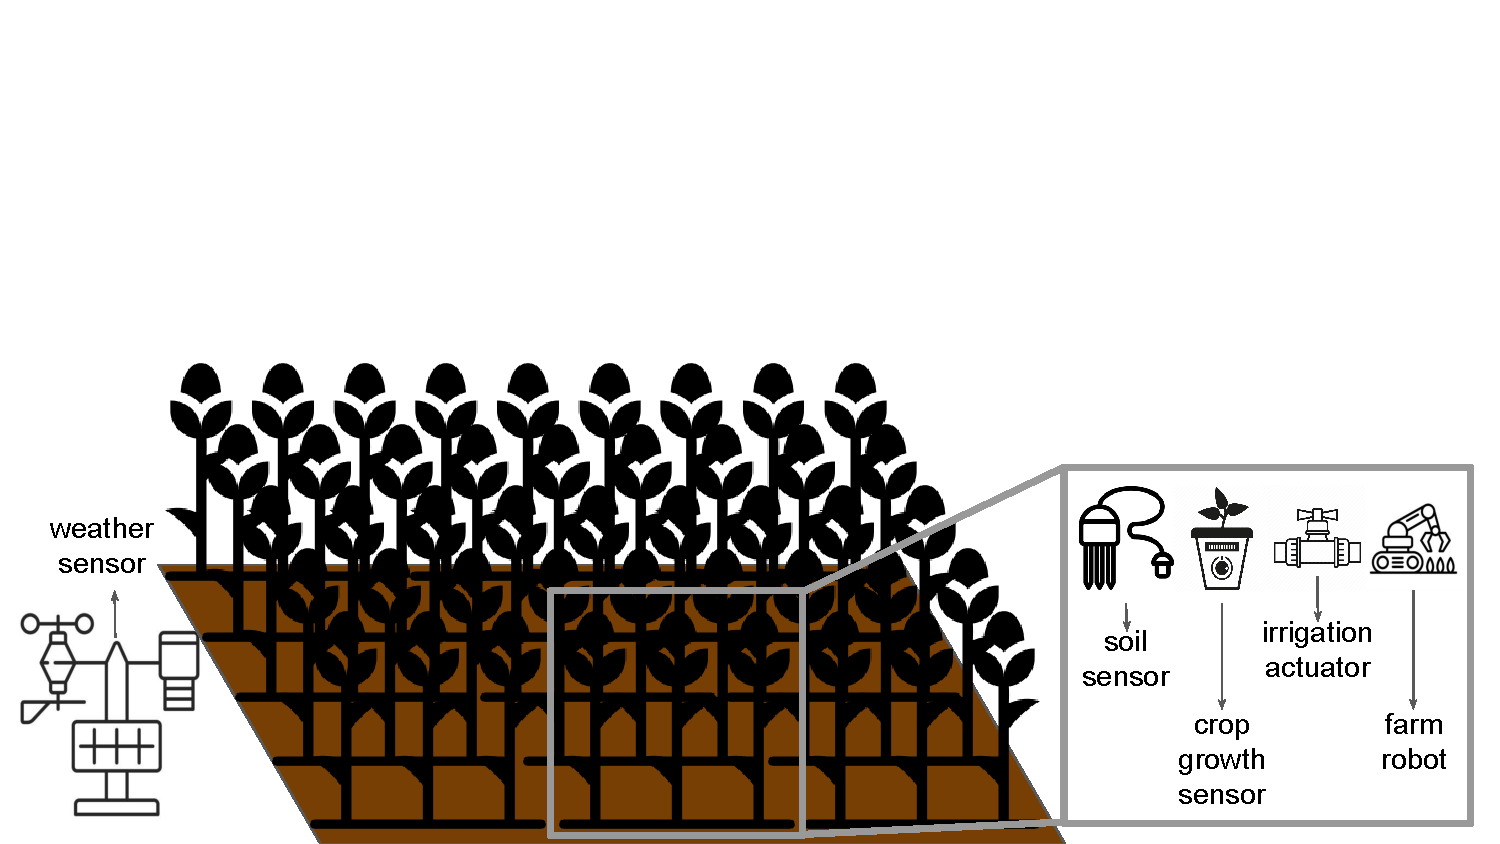
\includegraphics[width=\textwidth]{CoMesh/figures/intro/smart-farm.pdf}
        \caption{\it \small {Smart Farm.}}
        \medskip
        \label{comesh:fig:smart-farm}
    \end{subfigure}
    \begin{subfigure}{0.49\linewidth}
        % \vspace{0.2cm}
        \centering
        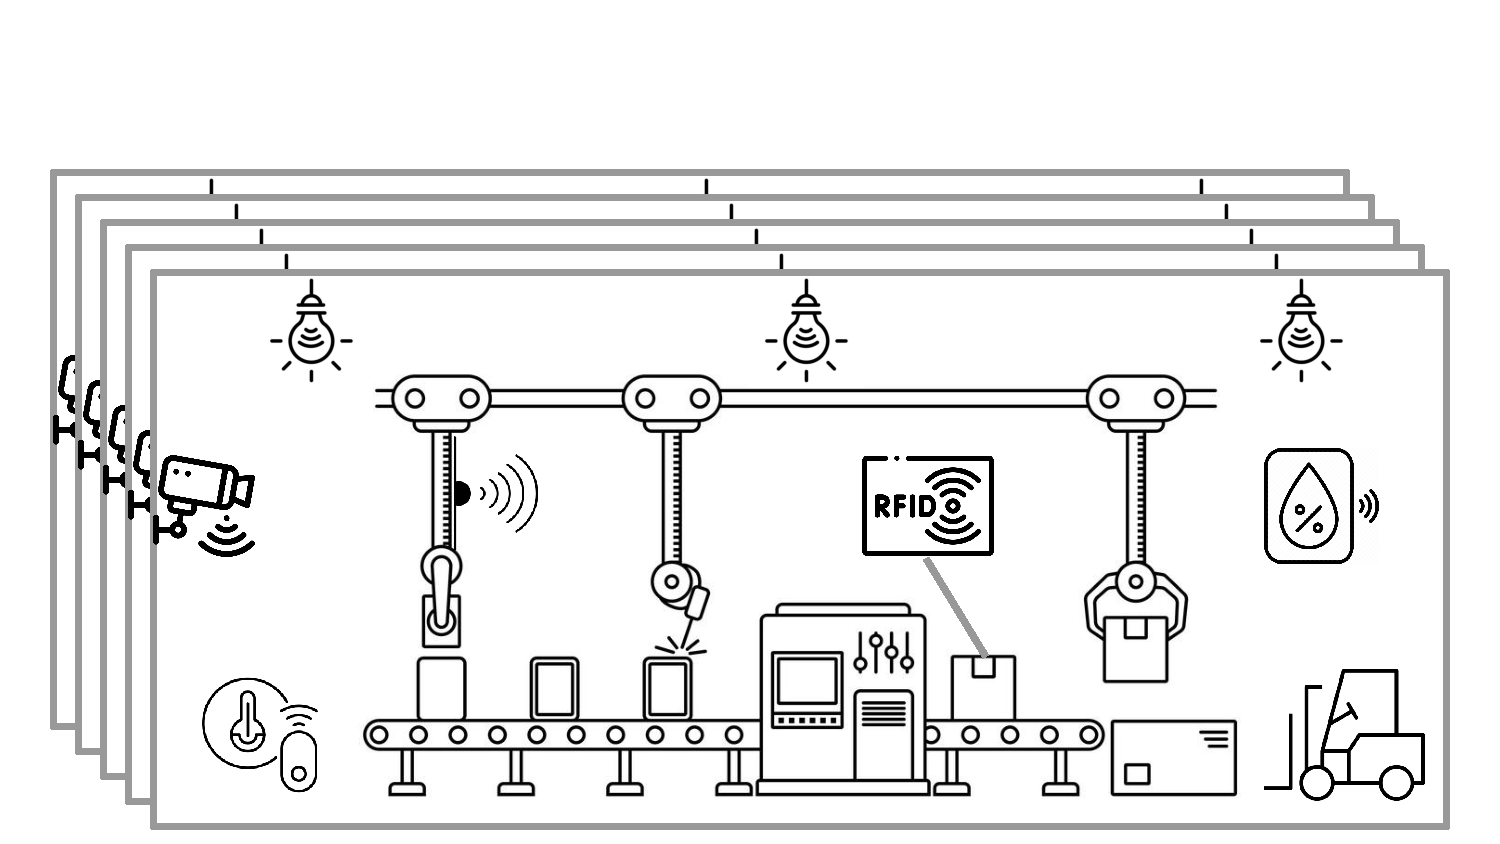
\includegraphics[width=\textwidth]{CoMesh/figures/intro/smart-factory.pdf}
        \caption{\it \small {Smart Factory.}}
        % \medskip
        \label{comesh:fig:smart-factory}
    \end{subfigure}
    \caption{\it \small {Three Commercial Edge Settings:
    (a)  \Bldg~\cite{Memoori}, (b)  \Grid~\cite{SMG21}, (c) Smart  Factory~\cite{lampropoulos2019internet}. We later use the \Bldg{} map from (a) and \Grid{} from (b) to drive experiments. }
    }
    \label{comesh:fig:IoTsetting}
\end{figure}


{\noindent \bf Sense-Trigger-Actuation of Routines:} Sitting {\it above} this mesh network is the  {\it control plane}---this typically needs to execute three kinds of actions:
{\it Sense-Trigger-Actuate} (or STA). The control plane needs to first {\it sense}: continuously collect measurements from multiple devices. Applications specify predicates, which are arbitrary Boolean clauses involving multiple device readings. Whenever a predicate is satisfied, the control plane  needs to {\it trigger} a programmed
series of actions, sending
commands to several devices. Third, because some of these actions may be long-running (e.g., mechanical movements, repetitive actions, or time-based actions such as water sprinklers), the control plane needs to initiate and monitor {\it actuation} of these commands (at multiple devices)  quickly and efficiently. The key challenge is to actuate in an order that {\it avoids conflicting actions on devices~\cite{Transactuations, Safehome}}.

This STA abstraction is commonly programmed via {\it routines}, available in Amazon Alexa \cite{Alexa}, Google Home \cite{GoogleHome}, etc. A  routine is a sequence of {\it commands} that actuates multiple devices,  wherein each command executes an action on one device. Multiple routines may be active at any given time, while others remain dormant (waiting to be triggered). A routine may be triggered either based on sensor values (Boolean predicate), or at particular times, or a combination of these, or manually by a human.

This paper focuses on management of such routine-based workloads running over large commercial edge IoT meshes. \Cref{comesh:fig:IoTsetting} shows three emerging edge mesh scenarios---a smart building, a smart farm, and a smart factory.
Some examples of routines follow. A  smart office will have routines running day and night, e.g., to: (i) raise and lower shades and thermostat, in response to sunlight and temperature; (ii) change interior lighting as a function of occupancy; (iii) enable security cameras and lock gates at 9 pm. 
A smart farm has routines that: (iv) water dry areas of the farm when soil sensors detect dryness below a threshold; (v) trigger robots to inspect crops. 
Routines might be triggered by sensors, time (fixed or periodic), or humans. 
For a routine that is sensor- and/or time-triggered, its trigger clauses need to be monitored continually so that after the trigger becomes true, the routine starts execution {\it quickly}. 

Another key  challenge in scheduling these routines is to avoid
{\it conflicts among routines}, i.e., {\it two routines that actuate intersecting sets of devices should not be allowed to execute concurrently, but instead be executed serially}. Handling conflicts is an important and difficult problem, but existing solutions~\cite{Safehome} are centralized and hub-based.  

{\noindent \bf Towards Cloudless and Hubless STA Operations: }  
Commercial edge settings have a strong requirement of uninterrupted operation. This has led to recent efforts that build ``Cloudless IoT'' solutions across both industry~\cite{Thingsquare}
and open source~\cite{HACloudless,csa2025matter}.
Benefits of cloudlessness include: lower latency, stability (cloud outages do not affect local operations), persistence (no effect of changing cloud services and APIs), lowered cost for providers (no cost of running on cloud services\footnote{Provider cost for a customer with 500 devices pinged every second, plus routine actuation, can be as high as \$2500 per month~\cite{AzureIoTHub}.}), 
% 2 msgs * 24 hours * 60 mins * 60 secs * 1000 ms / 40ms = 4,320,000 msgs per day
% 2 msgs * 24 hours * 60 mins * 60 secs * 1000 ms / 2ms = 86,400,000 msgs per day
% Azure IoT hubs pricing:
% tier S2 charges $250 per month for up to 6,000,000 daily messages of 4 KB size
% tier S3 charges $2,500 per month for up to 300,000,000 daily messages of 4 KB size
and keeping operations+data private and local.


\begin{figure}[t]
    \centering
    \begin{subfigure}[b]{0.4\linewidth}
        \centering
        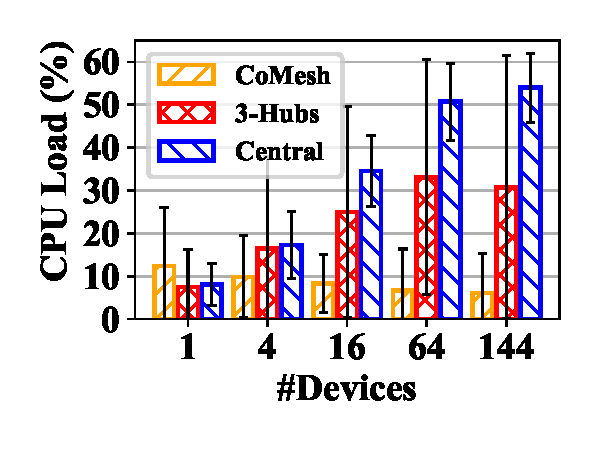
\includegraphics[width=\textwidth]{CoMesh/figures/intro/CPU_cmp_xdev_bar.pdf}
        \caption{ \small \it Fixed: 20 total routines.
        }
        \label{comesh:subfig:cpu-central}
    \end{subfigure}
    \hspace{0.5cm}
    \begin{subfigure}[b]{0.4\linewidth}
        \centering
        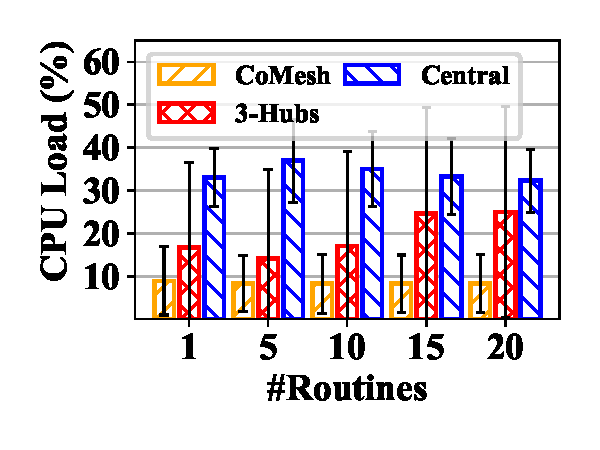
\includegraphics[width=\textwidth]{CoMesh/figures/intro/CPU_cmp_xrtn_bar.pdf}
        \caption{\small \it Fixed: 16 total devices.}
        \label{comesh:subfig:cpu-cmp}
    \end{subfigure}
    \caption{\small \it 
    Raspberry Pis: Our decentralized \sysname{} reduces CPU utilization significantly compared to the centralized Hub and 3-Hubs.}
    \medskip
    \label{comesh:fig:resources}
\end{figure}

A cloudless commercialized edge has two possible design paths:
(1) a local hub-based solution, or (2) a {\it hubless} (fully-decentralized)  solution. Preliminary work exists on the former~\cite{HACloudless}, and the latter~\cite{rivulet}.
Rivulet~\cite{rivulet} is the first {\it decentralized} (hubless) IoT solution we know
of, and it is scoped on data streams and individual commands,
\textit{not} routines.
No existing system
handles inter-routine conflicts, \textit{and} with decentralization.
Our paper takes the next big step in making cloudless commercial edges hubless and fully decentralized. The cloudless+hubless approach addresses concerns of the hub being overwhelmed
(\Cref{comesh:fig:resources}), and being susceptible to unreliability~\cite{moore2020iot} and cloud outages~\cite{gcloud-down1}.
%
\Cref{comesh:fig:resources}(a, b), done with Raspberry Pis, shows that with more devices (i) CPU load on the {central hub} rises rapidly and crosses 50\% at just 64 devices, (ii) even with 3 central hubs sharing the load, the CPU load is high (30\%) and has high variance. The per-device CPU load is reduced by over 6$\times$ (beyond 64 devices, or 15 routines) vs the 3-hubs by our decentralized solution (\sysname), at 5.2\%-12.4\%, and it scales (remains flat). Regardless of load concerns, hubless solutions are paramount due to needs of user privacy (of data \& operations), cloud outage resilience, and lowering cloud costs.


\renewcommand{\arraystretch}{1.2}

\begin{table}[t]
\centering
\caption{\small \it N-hubs vs.\ \sysname{} design trade-offs.}
    \bigskip
\label{comesh:tab:n-hubs-vs-comesh}
\footnotesize
% \tagpdfsetup{table/header-rows={1},table/header-columns={1}}
\tagpdfsetup{table-tagging=false}
\begin{tabularx}{\columnwidth}{@{}>{\raggedright\arraybackslash}p{2.5cm}
                               @{}>{\raggedright\arraybackslash\hsize=0.97\hsize}X
                               @{}>{\raggedright\arraybackslash\hsize=1.03\hsize}X@{}}
\hline
\textbf{Property} & \textbf{N-Hubs (Sharded/Hierarchical)} & \textbf{CoMesh (this paper)} \\
\hline\hline

% Complexity (1 pair)
\textbf{\textit{Complexity}} &
Simpler at small scale &
Complex, but with correctness proofs \\
\hline

% Device Impact (1 pair)
\raggedright\textbf{\textit{Device Impact}}
& \multirow{2}{5cm}{Processing only at hubs} &
\multirow{2}{6cm}{Devices process, but load is balanced} \\
\hline

% Deployment, Setup & Scalability (4 pairs)
\multirow{6}{2.5cm}{\raggedright\textbf{\textit{Deployment, Setup \& Scalability}}} &
Static sharding & 
Spatial rebalancing via \kgroups \\
\cline{2-3}
& Manual reconfig via static sharding; dynamic reconfig needs \sysname-like logic &
\multirow{2}{6cm}{Dynamically reconfigurable with churn} \\
\cline{2-3}
& Hubs can overload &
Temporal rebalancing smooths long-term load \\
\cline{2-3}
& Scalability limited by \#hubs \& inter-hub coordination &
\multirow{2}{6cm}{Scales well} \\
\hline

% Fault Tolerance (1 pair)
\raggedright\textbf{\textit{Fault Tolerance}} &
Limited resilience; hub faults disrupt many routines &
Tolerates up to $f$ device faults via quorums/migration \\
\hline

% Resource Overhead (1 pair)
\textbf{\textit{Resource Overhead}} &
\multirow{2}{6cm}{Preferable for small-scale setups} &
Preferable for larger on-field setups with many devices \\
\hline
\end{tabularx}
\end{table}

\Cref{comesh:tab:n-hubs-vs-comesh} details the tradeoffs between \sysname{} and an alternate solution that might use multiple (N) hubs to coordinate device and routine actions. Overall, N-hubs can be simpler as it uses static sharding, but this requires manual reconfiguration, e.g., when devices are added/removed, hubs are added/removed. \sysname{} dynamically reconfigures and scales arbitrarily, but comes with some level of complexity; we balance this complexity with proofs of correctness. At its core, however, autonomous coordination among N hubs {\it will} require coordination similar to \sysname's mechanisms. In other words, one can reuse \sysname's core techniques to also implement a solution with N hubs, and be assured of correctness.


A cloudless+hubless STA solution requires that all actions: 
(i) operate {\it over the local edge mesh}, (ii)  remain {\it local}, without requiring a connection to the cloud, and (iii) maintain {\it fault-tolerance\footnote{While this paper only deals with crash failures, our decentralized approaches spread the attack surface and are more secure than a centralized cloudless solution. Security is beyond the scope of this paper.}} in spite of local device failures.  



\noindent {\bf Contributions: } We present \sysname, the first system to realize
a {\it fully decentralized} (i.e., hub-less and local)    control plane for  monitoring and management of  routines
over large edge meshes. The contributions of this paper are: 
\begin{itemize}
    \item Design and implementation of \sysname, using 
    a novel combination of techniques: 
    (1)
    distributed sense, trigger, and actuate
    operations over both space and time; 
    (2) fast coordination via zero-message exchange and quorum-based protocols; (3) distributed coordination to ensure conflict-free actuation of routines; and (4) locality-based hashing (LSH) to keep communication local. While some of these techniques are known, \sysname{} is unique in the way it combines them to solve  STA challenges.
    \item Our Raspberry Pi-4 deployment experiments and
    simulations, using real building maps and real
    routine workloads, show
    \sysname{} is scalable, efficient,  fault-tolerant, and fast.
\end{itemize}
Our source code and datasets are available at \href{dprg.cs.uiuc.edu/traces/go.php?id=42}{https://dprg.cs.uiuc.edu/traces/go.php?id=42} and \href{dprg.cs.uiuc.edu/traces/go.php?id=43}{https://dprg.cs.uiuc.edu/traces/go.php?id=43}.

\begin{figure}[t!]
    \centering
    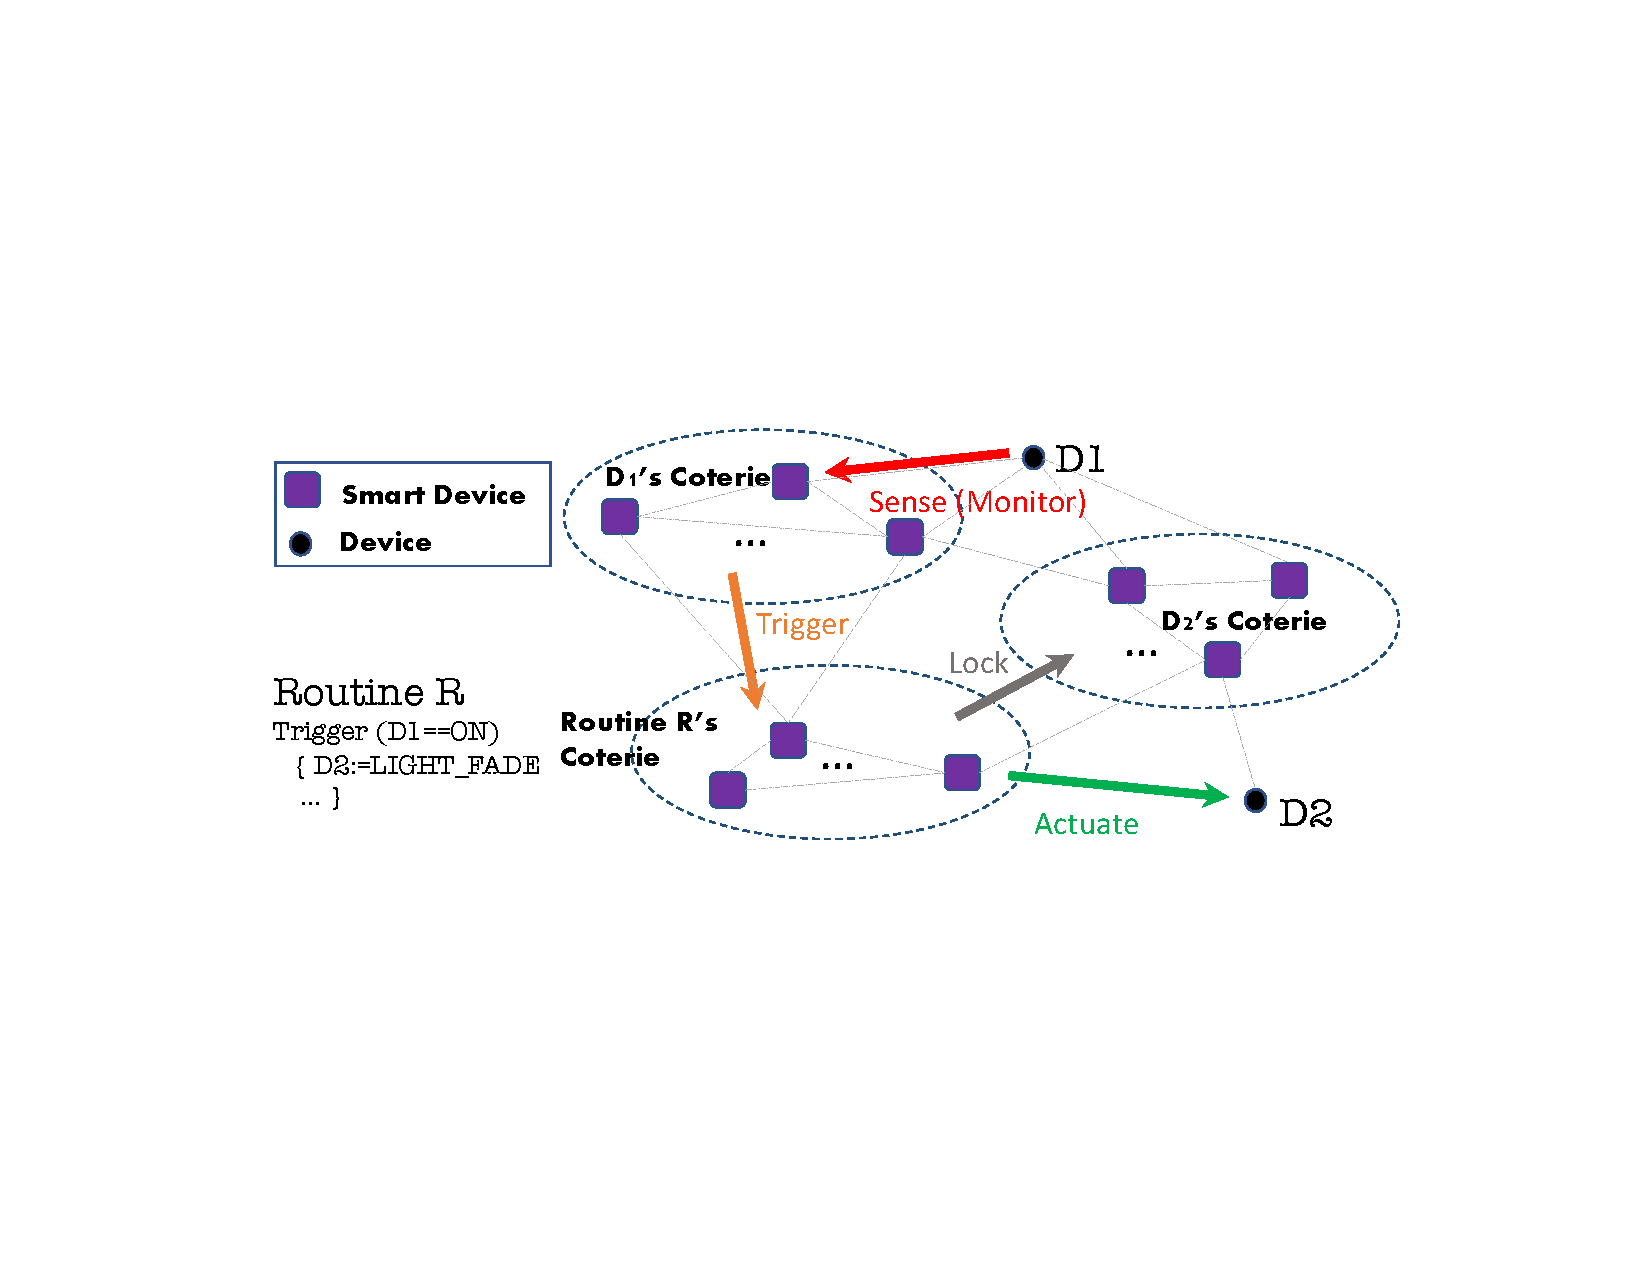
\includegraphics[width=0.8\linewidth]{CoMesh/figures/intro/Coteries.pdf}
    \caption{\small \it Control Flow of \sysname's Sense-Trigger-Actuate Actions. Ad-hoc network links are shown in the background. (For simplicity, all \kgroups{} are shown as hyper-local.)
    }
    \medskip
    \label{comesh:fig:coteries}
\end{figure}

\subsection{Challenges and \sysname's Overview}
\label{comesh:sec:motivation}

\noindent {\bf Challenges of Decentralization: } 
\sysname's goal is to design a hub-less, fully decentralized, local,  STA management system that relies on neither a single central hub nor a cloud. \sysname{} contains {\it local} distributed protocols running among smart devices which have compute and memory resources (other simple devices without such resources may also co-exist)---\sysname{} requires only a fraction of devices to be smart. Smart devices may include 
IoT devices, Raspberry Pis, home hubs, handheld devices (phones, tablets), etc.

\sysname{} has to tackle five major challenges: (1) {\it fully decentralized} operation: sensing (monitoring), triggering, and actuation of routines, without any reliance on centralization;
(2) {\it conflict-free} actuation of routines: no  two routines that actuate intersecting sets of devices should be simultaneously active~\cite{Transactuations, Safehome};
(3) {\it load balance}: of STA overhead both across devices and across  time; (4) {\it robustness}: {to tolerate failures} of devices; and (5) {\it physical awareness:} network  load that is    {aware of the physical layout of devices}. 

\noindent {\bf \sysname's Overview:} 
Now we summarize key internal components of \sysname. 
Internally \sysname{} balances the STA load across both {\it space and time}. 
Spatial balancing divides the STA load (of an erstwhile hub) across multiple smart devices. Since some devices may be more popular (appear in more routines), and some routines run more frequently, temporal balancing spreads the load from these ``popular'' devices and routines across \smarts. 
\sysname{}  implements such balancing by using {\it \kgroups}---subgroups of smart devices responsible for devices
and routines. For {\it Spatial balancing} there is: (i) a separate \kgroup{} for each device, responsible for continually sensing that device,
and (ii) a \kgroup{} per routine to handle its triggering, actuation, and conflict-free execution. \Cref{comesh:fig:coteries} depicts that a routine's \kgroup{} coordinates with the \kgroups{} of all its trigger-clause devices as well as \kgroups{} of its actuated devices, in order to ensure conflict-free operation of routines.  To reduce coterie count further, \sysname{} multiplexes multiple devices/routines into the same \kgroup. {This means that a given device may {\it belong} as a member of multiple \kgroups{}, but there is still exactly one coterie to monitor a given device, and exactly one coterie to manage a given routine.}

\Kgroup{} selection comes in two flavors---hashing-based,  and locality-sensitive-hashing based which keeps \kgroup{} communications local. Within each \kgroup{} we carefully design fast and cheap IoT coordination via quorum-based agreement, leader election, and tolerance to \kgroup{} leader and member failures. Specifically, to tolerate $f$ failures in the system, it is sufficient for each \kgroup{} to contain ${k=}(2f+1)$ members. 


{\it Temporal balancing} proactively migrates   membership of \kgroups{} over time across nodes. To make it fast and cheap, \sysname{} uses {\it zero-message exchange} protocols for
selection---``zero-message'' means that any smart device (in the fast path), without exchanging any messages, can calculate the current membership of any \kgroup{}.
This mechanism uses zero foreground messages, relying instead on constant background bandwidth from the weakly-consistent membership protocol. This reduces both complexity and convergence time.
